\documentclass{beamer}
\usetheme{CambridgeUS}
\usecolortheme{dolphin}

\usepackage[greek,english]{babel}
\usepackage[OT2,OT1]{fontenc}
\usepackage[utf8]{inputenc}

\usepackage{hyperref}
\hypersetup{colorlinks=true,breaklinks=true,linkcolor=,urlcolor=blue}

\usepackage{geometry}
\usepackage{enumerate}
\usepackage{multirow}
\usepackage{multicol}
\usepackage{ulem}
\usepackage{graphicx}
\usepackage{subfigure}
\usepackage{amsmath}
\usepackage{amssymb}
\usepackage{mathrsfs}
\usepackage{latexsym}
%\usepackage[scheme=plain]{ctex}
\usepackage{tikz}
\usepackage{verbatim}

% use xpatch to remove frame of venndiagram
\usepackage{venndiagram}
\usepackage{xpatch}
\tikzset{
  vennframe/.style={draw=none} % define a new style for the frames
}
\makeatletter
\xpatchcmd{\endvenndiagram3sets}
{\draw (0,0) rectangle (\@venn@w,\@venn@h);} % replace this
{\draw [vennframe] (0,0) rectangle (\@venn@w,\@venn@h);} % with this -- add the style
{}{}

\xpatchcmd{\endvenndiagram2sets}
{\draw (venn bottom left) rectangle (\@venn@w,\@venn@h);}
{\draw [vennframe] (venn bottom left) rectangle (\@venn@w,\@venn@h);}
{}{}
\makeatother

\title{VE414 Presentation}
\author{Group 9}
\date{August 5, 2019}

\begin{document}

\maketitle


\section{Density Estimation}

\begin{frame}{Overview of Density Estimation}
    \begin{itemize}
        \item Known: Many records of the number of Tayes
        \item Required: Estimation of Tayes in the Forest
        \item Solution: \begin{itemize}
            \item Divide map into grid ($107\times 107$)
            \item Calculate the density on the grid according to the records within 1 meter
            \begin{itemize}
                \item For two records using \textit{density estimation of two intersected circles}
                \item For more than two records taking the mean of the estimation
            \end{itemize}
            \item Tayes sample according to the density
        \end{itemize}
    \end{itemize}
    \begin{figure}[H]
        \centering
        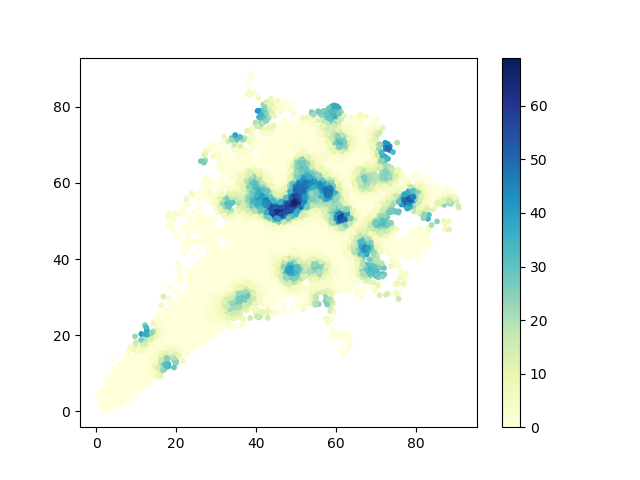
\includegraphics[scale=0.25]{ag.png}
        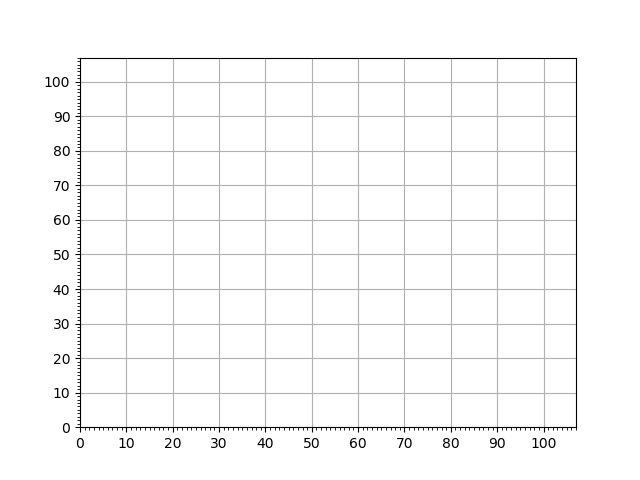
\includegraphics[scale=0.25]{grid.png}
    \end{figure}
\end{frame}

\begin{frame}{Density Estimation of two Intersected Circles}

Suppose there are two detected circles which intersect with each other. We only know
$$\text{Tayes}[A=A'\cup C]=a,\quad\text{Tayes}[B=B'\cup C]=b$$
from the magic of Hermione.

\begin{center}
    \begin{venndiagram2sets}[labelOnlyA={A'}, labelOnlyB={B'}, labelA={A}, labelB={B}, labelAB={C}, overlap=0.75cm, hgap=0cm, vgap=0cm, radius=1cm]
        \fillACapB
    \end{venndiagram2sets}
\end{center}


If Tayes are (approx) uniformly distributed in a circle, and $S_A\approx S_B$, $a\approx b$,
$$\quad\text{Density}[C]\approx\left(\frac{a}{S_A}+\frac{b}{S_B}\right)/2,\quad c=\text{Density}[C]\cdot S_C,$$
$$\text{Density}[A']\approx\frac{a-c/2}{S_A-S_C},\quad\text{Density}[B']\approx\frac{b-c/2}{S_B-S_C}.$$    

\end{frame}

\begin{frame}
    However, these conditions don't always hold, so we need to extend our model. Keep the assumption that Tayes are uniformly distributed in a circle, the number of Tayes $x$ in area $C$ should follow binomial distributions $B(a,p_a=S_C/S_A)$ and $B(b,p_b=S_C/S_B)$ in two circles.
    $$P[X=x]=\binom{a}{x}p_a^x(1-p_a)^{a-x}\binom{b}{x}p_b^x(1-p_b)^{b-x},$$
    $$P_x=P[X=x]\Bigg/\sum_{i=0}^{\min\{a,b\}}P[X=i],$$
    $$\text{Density}[A']=\frac{1}{S_A'}\sum_{i=0}^{\min\{a,b\}}(a-i)P_i,\quad\text{Density}[B']=\frac{1}{S_B'}\sum_{i=0}^{\min\{a,b\}}(b-i)P_i,$$
    $$\text{Density}[C]=\frac{1}{S_C}\sum_{i=0}^{\min\{a,b\}}iP_i.$$
\end{frame}



\section{Guassian Mixture Model}
\begin{frame}{Guassian Mixture Distribution}
    \begin{itemize}
        \item Assumption: The distribution of the fruits from a tree follows the \textit{Bivariate Gaussian Distribution}. 
        \item The distribution of Tayes on the ground $\sim$ Guassian Mixture Distribution
        $$ p(x)=\sum\limits_{k=1}^K\pi_k N(x|\mu_k,\Sigma_k) $$ where $\sum\limits_{k=1}^K\pi_k = 1$. $K$ is the number of trees, $\mu_k$ is the position of the tree, $\pi_k$ and $\Sigma_k$ determines some unique properties of a tree.
        \item Aim: Fit Guassian Mixture Model(GMM) with Tayes Samples
    \end{itemize}
\end{frame}

\begin{frame}{Fit GMM with Expectation-Maximization algorithm (EM)}
    \begin{itemize}
        \item E-step: calculate the posterior probabilities for $k\in\{1,\cdots,K\}, n\in\{1,\cdots,N\}$ $$ \gamma_{nk}=p(k|x_n)=\dfrac{\pi_k\mathcal{N}(x_n|\mu_n,\Sigma_n)}{\sum_{j=1}^K\pi_j\mathcal{N}(x_n|\mu_j,\Sigma_j) } $$
        \item M-step: calculate the value for $\pi_k,\ \mu_k,\ \Sigma_k$
        \begin{align*}
            \mu_k' & = \dfrac{\sum_{n=1}^N\gamma_{nk}x_n}{\sum_{n=1}^N\gamma_{nk}}\\
            \Sigma_k' & = \dfrac{\sum_{n=1}^N\gamma_{nk}(x_n-\mu_k')(x_n-\mu_k')^T}{\sum_{n=1}^N\gamma_{nk}}\\
            \pi_k' &= \dfrac{\sum_{n=1}^N\gamma_{nk}}{N}
        \end{align*}
    \end{itemize}
\end{frame}
\begin{frame}
    \begin{itemize}
        \item Loop until log likelihood convergence:
        $$ \text{ln}p(X|\mu,\Sigma,\pi) = \sum_{n=1}^Nln\{\sum_{k=1}^K\pi_k\mathcal{N}(x_n|\mu_k,\Sigma_k)\} $$
        \item Pick a k = $\arg\limits_k\min$ BIC(Bayesian Information Creterion):
        $$ BIC = -2ln(L)+ln(N)*K $$
    \end{itemize}
\end{frame}
% BIC的图和最后选定K

\begin{frame}{Generalize tree distribution to unobserved areas}
    \begin{itemize}
    \item Assumptions
        \begin{itemize}
            \item Assumption 1: The number of trees in each grid of a certain size follows Poisson distribution with parameter $\lambda$.
            \item Assumption 2: In each grid, the trees are located uniformly.
        \end{itemize}
    \item Estimate $\lambda$
        $$L(\lambda)=\ln\prod f(k_i|\lambda)=-n\lambda-\sum\ln(k_i!)+(\sum k_i)\ln\lambda$$
        $$\hat{\lambda}_{MLE}=\frac{1}{n}\sum k_i$$
    \item Random Generation
        \begin{enumerate}
            \item For each unobserved grid, sample the number of trees in it according to the estimated Poisson distribution
            \item For grids with trees, randomly generate positions for these trees
        \end{enumerate}
    \end{itemize}
\end{frame}

\begin{frame}{Result}
    \begin{itemize}
    \item Total estimated number of trees in the forest: 25 + 79 = 104
    \item An example of possible tree positions
    % scatter plot of tree positions
    \begin{figure}[H]
        \centering
        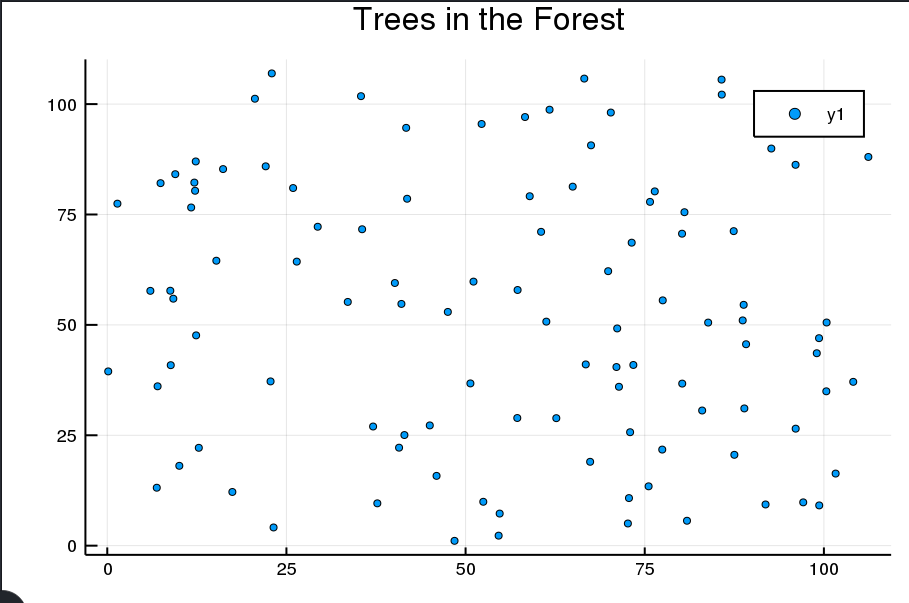
\includegraphics[scale=0.4]{final.png}
    \end{figure}
    \end{itemize}
\end{frame}

\end{document}
